
龙芯3A是龙芯多核处理器系列的第一款产品,是一个配置为单节点4核的龙芯3号处理器,采用65nm工艺制造,最高工作主频为1GHz,主要特征如下:

\begin{itemize}
\item{}片内集成四个64位的四发射超标量GS464高性能处理器核;
\item{}每个处理器核包括2个全流水的64位双精度浮点乘加部件;
\item{}每个处理器核包含64KB数据Cache和64KB的指令Cache;
\item{}片内集成四核共享的4MB二级Cache;
\item{}通过目录协议维护多核及I/O DMA访问的Cache一致性;
\item{}片内集成2个64位400MHz的DDR2/3控制器;
\item{}片内集成2个16位800MHz的HyperTransport控制器;
\item{}每个16位的HT端口拆分成两个8路的HT端口使用;
\item{}片内集成32位100MHz PCIX/66MHz PCI;
\item{}一个LPC、两个UART、1个SPI、16路GPIO接口;
\item{}采用128位AXI接口的交叉开关网络。
\end{itemize}

\begin{figure}[H] 
  \centering
  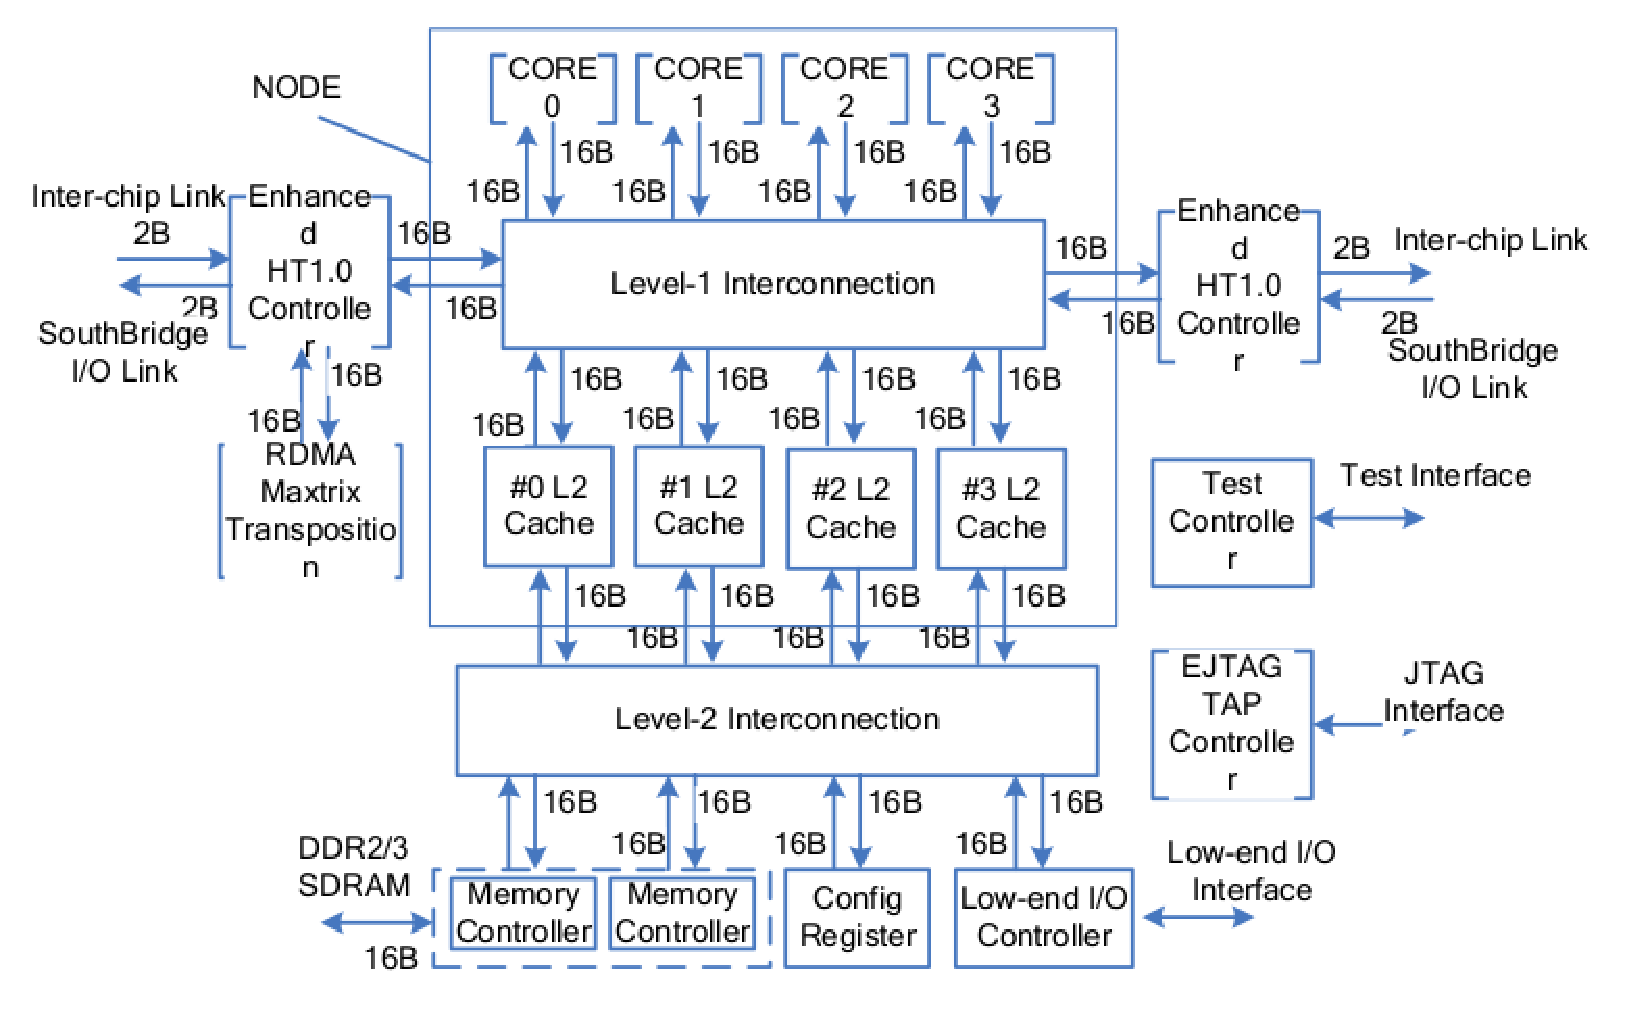
\includegraphics[width=10cm,height=6cm]{figures/chap01/Loongson3A}
  \caption{龙芯3A芯片结构}
  \label{fig:loongson3a}
\end{figure}

龙芯3A号芯片整体架构基于两级互连实现,结构如图\ref{fig:loongson3a}所示。由于四核龙芯3A在单芯片只包含一个节点,不用跟其他结点互连,因此第一层互连采用6x6的交叉开关,用于连接四个CPU(作为主设备)、四个二级Cache 模块(作为从设备)、以及两个IO端口(每个端口使用一个Master和一个Slave)。X1连接的每个IO端口连接一个16位的HT控制器,每个16位的HT端口还可以作为两个8位的HT端口使用。 HT控制器通过一个DMA控制器和X1相连, DMA控制器负责IO的DMA控制并负责片间一致性的维护。龙芯3号的DMA控制器还可以通过配置实现预取和矩阵转置\cite{Loongson3A-Manual}。
